\documentclass[../../DD.tex]{subfiles}
\begin{document}
\newpage
\section{Relational Tables}
	The relational schema tables provide a logical representation of the domain modeled in the preceding ER diagram. It offers a structured view of the database schema.

    The relational schema tables define the structure and organization of the database, specifying the tables, columns, and relationships between them. Each table represents a distinct entity or concept in the domain, while the columns within the tables define the attributes or properties associated with those entities.
	
	\begin{figure}[h]
	    \centering
	    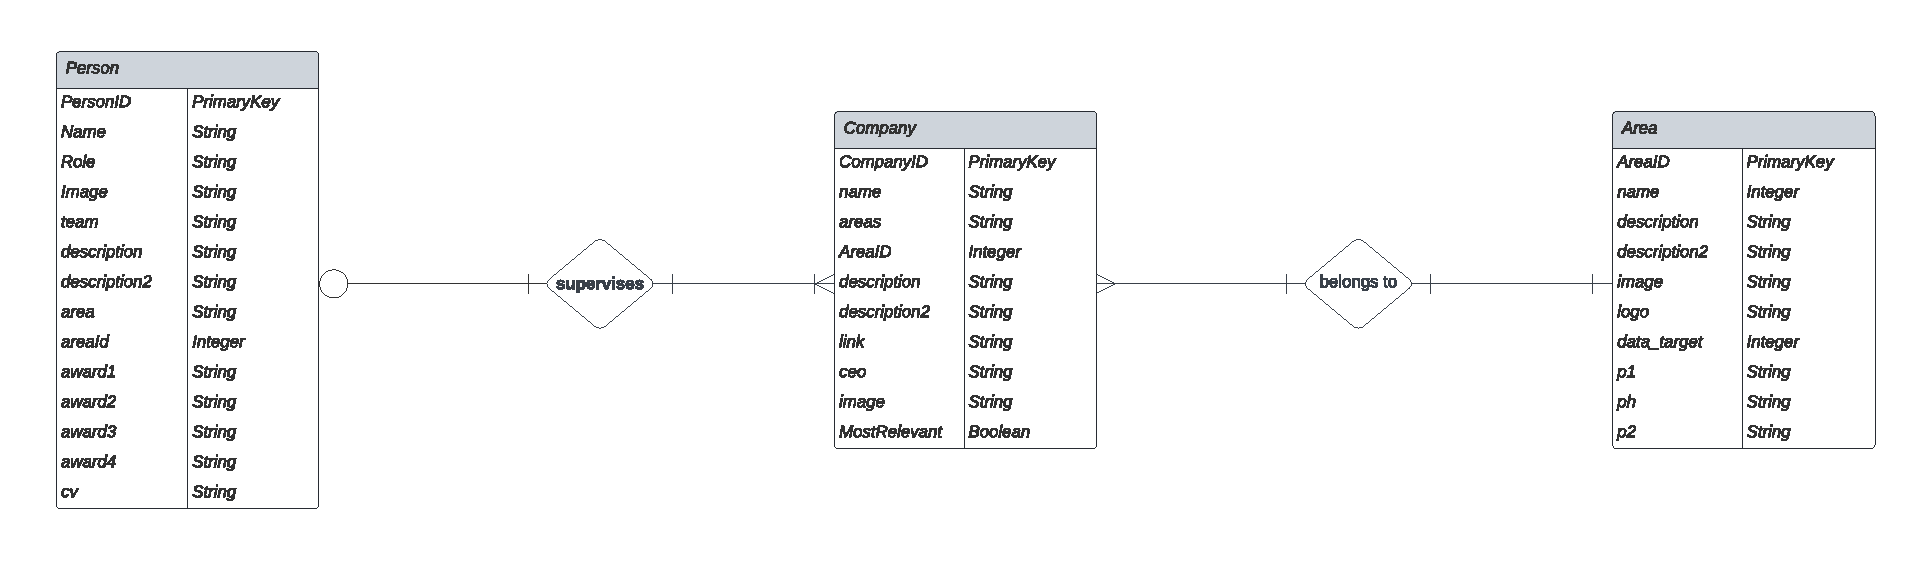
\includegraphics[width=\textwidth]{Images/Database/Database ER diagram (crow's foot).pdf}
	    \caption{Entity Relationship - Relational Tables}
	    \label{fig: ER}
	\end{figure}
	
\end{document}